\documentclass{beamer}

\usepackage{idrislang}
\usepackage{amsmath}
\usepackage{listings}
\usepackage{bussproofs}
\usepackage{tikz}
\usepackage{tikz-cd}

\usetheme{Szeged}
\usecolortheme{dolphin}

\title{An Introduction to Functional Programming}
\author{Thomas E. Hansen}
\institute{University of St Andrews}
\date{\today}

\begin{document}
\begin{frame}[plain]
  \titlepage
\end{frame}

\begin{frame}
  \frametitle{Overview}
  \tableofcontents
\end{frame}

\section{Introduction}
  \subsection{About}
  \begin{frame}
    \frametitle{About...}
    \begin{itemize}
      \item ... this talk
            \begin{itemize}
              \item This is a talk about functional programming
              \item It assumes no pre-existing knowledge
              \item I've tried to aim it at people with knowledge of imperative
                    languages
            \end{itemize}
      \item ... me!
            \begin{itemize}
              \item I'm Thomas
              \item I work with Edwin Brady
              \item I'm interested in formal methods, low-level programming,
                    making software provably robust/correct, etc
            \end{itemize}
    \end{itemize}
  \end{frame}

  \subsection{What do we mean by `functional'?}
  \begin{frame}
    \frametitle{What do we mean by `functional'?}
    \begin{itemize}
      \item As opposed to what? Non-functional?...
      \item Using \textit{functions}
        \begin{itemize}
          \item functions in the mathematical sense
          \item map inputs to outputs
        \end{itemize}
    \end{itemize}
  \end{frame}
  \begin{frame}
    \frametitle{Imperative vs Functional}
    \begin{itemize}
      \item Imperative
        \begin{itemize}
          \item Define a lot of details on \textit{how} to do things
          \item What to refer to memory as (e.g. variables and classes)
          \item How to operate on the memory, how to update it, etc
        \end{itemize}
      \item Functional
        \begin{itemize}
          \item Define the details of \textit{what} to do
          \item ``Given this input, the output looks like [...]''
          \item The idea being that humans are better at reasoning about this
          \item Leave the memory management and similar details to the programming
                language implementation and runtime
        \end{itemize}
    \end{itemize}
  \end{frame}

  \subsection{What FP doesn't have to be}
  \begin{frame}[fragile]
    \frametitle{It doesn't have to be like this}
    \begin{columns}[c]
      \tiny
      \column{0.5\textwidth}
        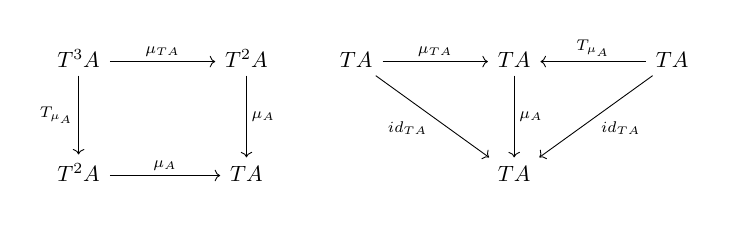
\begin{tikzpicture}
          \node[scale=0.8]{
          % drawn using https://tikzcd.yichuanshen.de/
          \begin{tikzcd}
            T^3A \arrow[dd, "T_{\mu_{A}}"'] \arrow[rr, "\mu_{TA}"] &  & T^2A \arrow[dd, "\mu_A"] & TA \arrow[rr, "\mu_{TA}"] \arrow[rrdd, "id_{TA}"'] &  & T²A \arrow[dd, "\mu_A"] &  & TA \arrow[lldd, "id_{TA}"] \arrow[ll, "T_{\mu_{A}}"'] \\
                                                                   &  &                          &                                                    &  &                         &  &                                                       \\
                                                                   T^2A \arrow[rr, "\mu_A"]                               &  & TA                       &                                                    &  & TA                      &  &
          \end{tikzcd}
          };
        \end{tikzpicture}

        \vspace*{6mm}

        {\small ``A monad is just a monoid in the category of endofunctors,
        what's the problem?''}

        \begin{prooftree}
          \AxiomC{$\Delta_0 \vdash \rho\ f \in (\pi x : S) \rightarrow T$}
          \AxiomC{$\Delta_1 \vdash \rho \pi\ S \ni s$}
          \BinaryInfC{$\Delta_0 + \Delta_1 \vdash \rho f s \in T[s: S/x]$}
        \end{prooftree}

      \column{0.5\textwidth}
        \centering
        \includegraphics[width=\textwidth]{stop-doing-type-theory.png}
        \tiny\color{gray}\url{https://twitter.com/jcreed/status/1367899760301137930}
    \end{columns}
  \end{frame}


\section{Getting started}

% TODO: there is an example here, but I need to fit it in
\iffalse
  \subsection{Example}
  \begin{frame}[fragile]
    \frametitle{Imperative programming}
    \begin{itemize}
      \item Summing the squares of numbers:
            {\footnotesize
            \begin{lstlisting}[language=java]
public int sumSquares(int n) {
  int sum = 0;
  for (int i = 0; i <= n; i++) sum += i*i;
  return sum;
}
            \end{lstlisting}
            }
      \item We have defined a lot of \textit{how}:
            \begin{itemize}
              \item create a variable \texttt{sum} with initial value 0
              \item update the memory referred to as `\texttt{sum}' to be the
                    contents of `\texttt{sum}', plus the contents `\texttt{i}'
                    times itself
              \item all the stuff about `\texttt{i}' in the `\texttt{for}' clause
            \end{itemize}
    \end{itemize}

  \end{frame}

  \begin{frame}[fragile]
    \frametitle{Functional programming}
    \begin{itemize}
      \item Summing squares in Idris:
            {\footnotesize
            \begin{idrislisting}
sumSquares : Int -> Int
sumSquares 0 = 0
sumSquares n = n*n + sumSquares (n - 1)
            \end{idrislisting}
            }
    \end{itemize}
  \end{frame}
\fi

\section{Concepts}
\subsection{Functions}

\end{document}
